\section{VALIDACIÓN DE RESULTADOS}

Como proyecto de ingeniería, se debe llevar a cabo un análisis de cumplimiento de los requerimientos del sistema desarrollado a través de métricas. Para la validación se van a evaluar las 
diferentes partes del trabajo.

Primeramente, a través del entrenamiento de la red neuronal, se ha buscado minimizar el error asociado a las \texttt{Bounding Boxes}, ya que el sistema usa esto como base para calcular movimientos. 
En este sentido, con el último conjunto de datos y 600 épocas, se han conseguido alcanzar un error de \texttt{0.2} y \texttt{0.9} en el conjunto de datos de entrenamiento y validación respectivamente, siendo 
este resultado uno de los mejores de todos los entrenamientos y con un conjunto de validación mucho más realista. Los resultados de la validación se pueden ver en la \autoref{fig:ValidacionRed}.

\begin{figure}[H]
    \centering
    \begin{subfigure}[b]{0.7\textwidth}
        \centering
        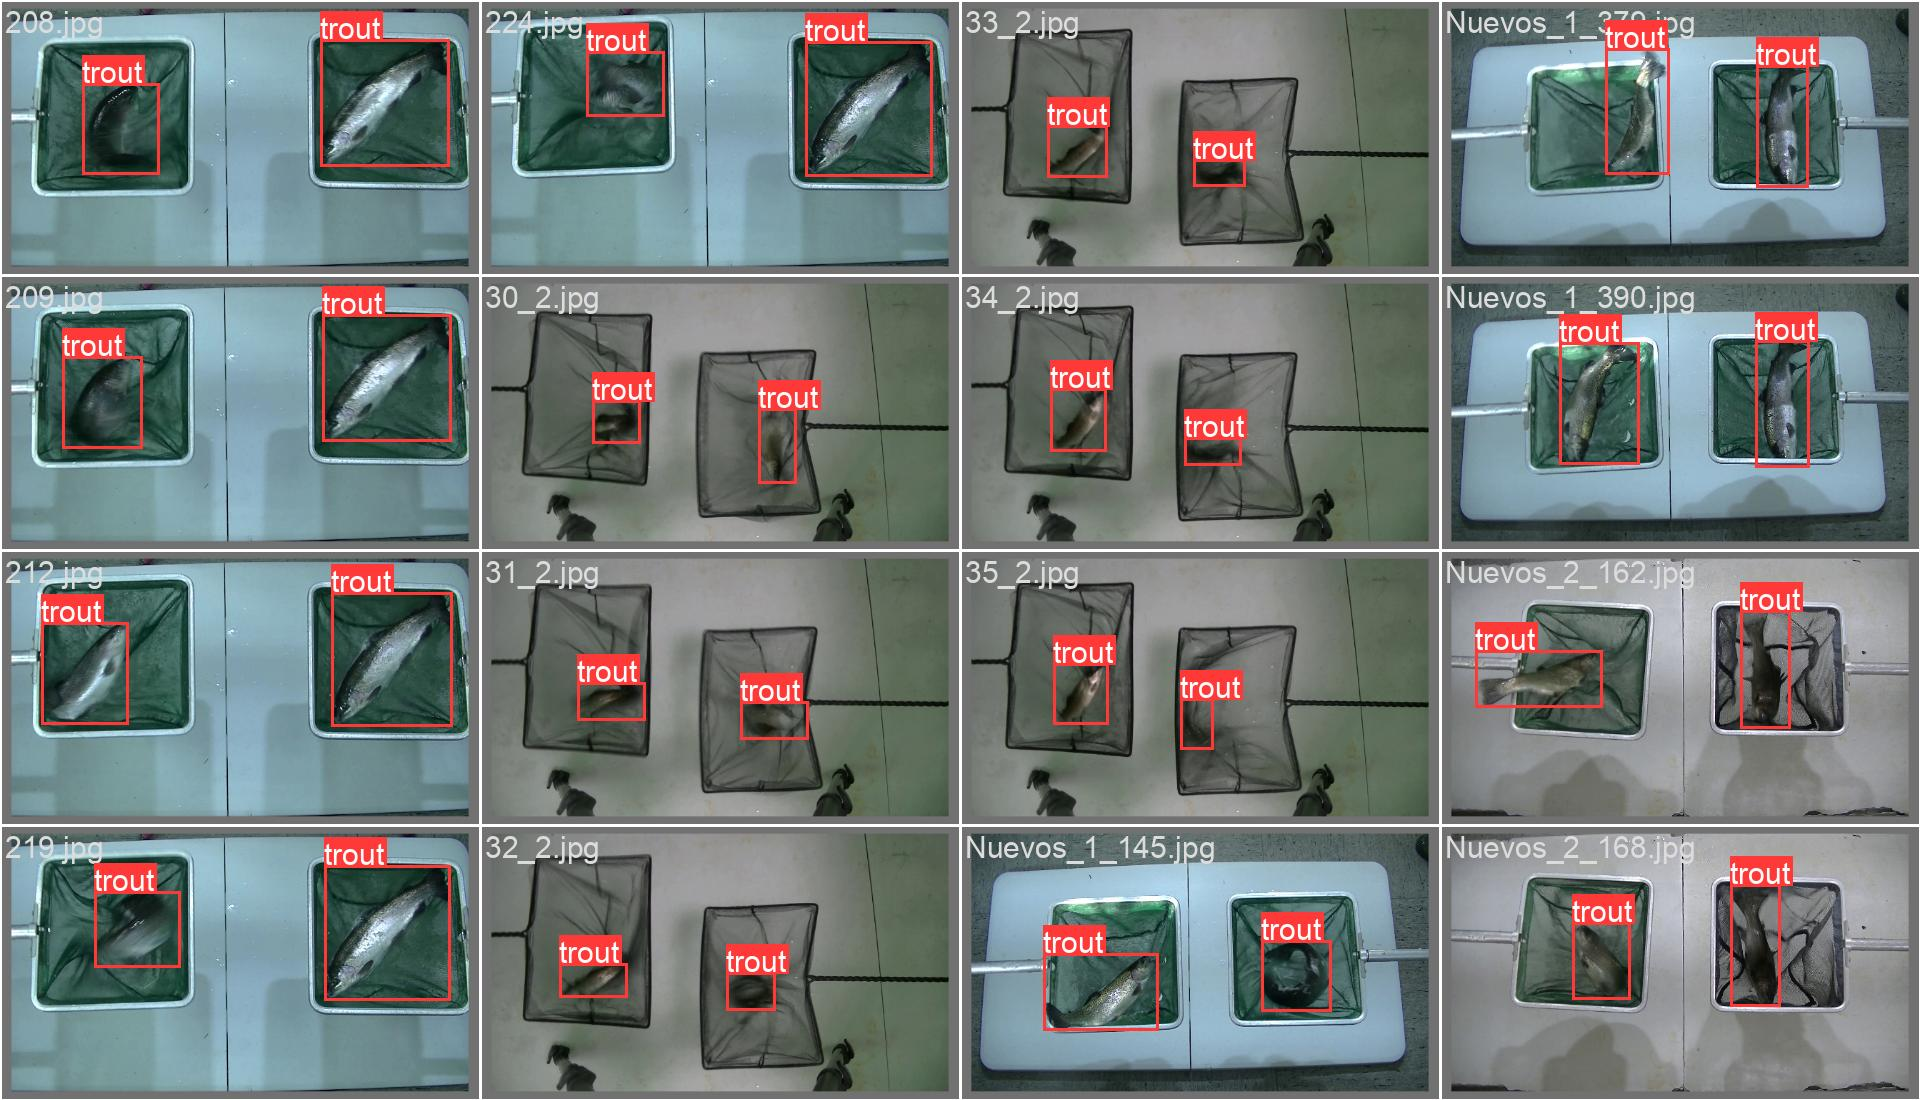
\includegraphics[width=0.95\textwidth]{images/7/labels.jpg}
        \caption{Etiquetas del conjunto de validación final}
    \end{subfigure}
    \begin{subfigure}[b]{0.7\textwidth}
        \centering
        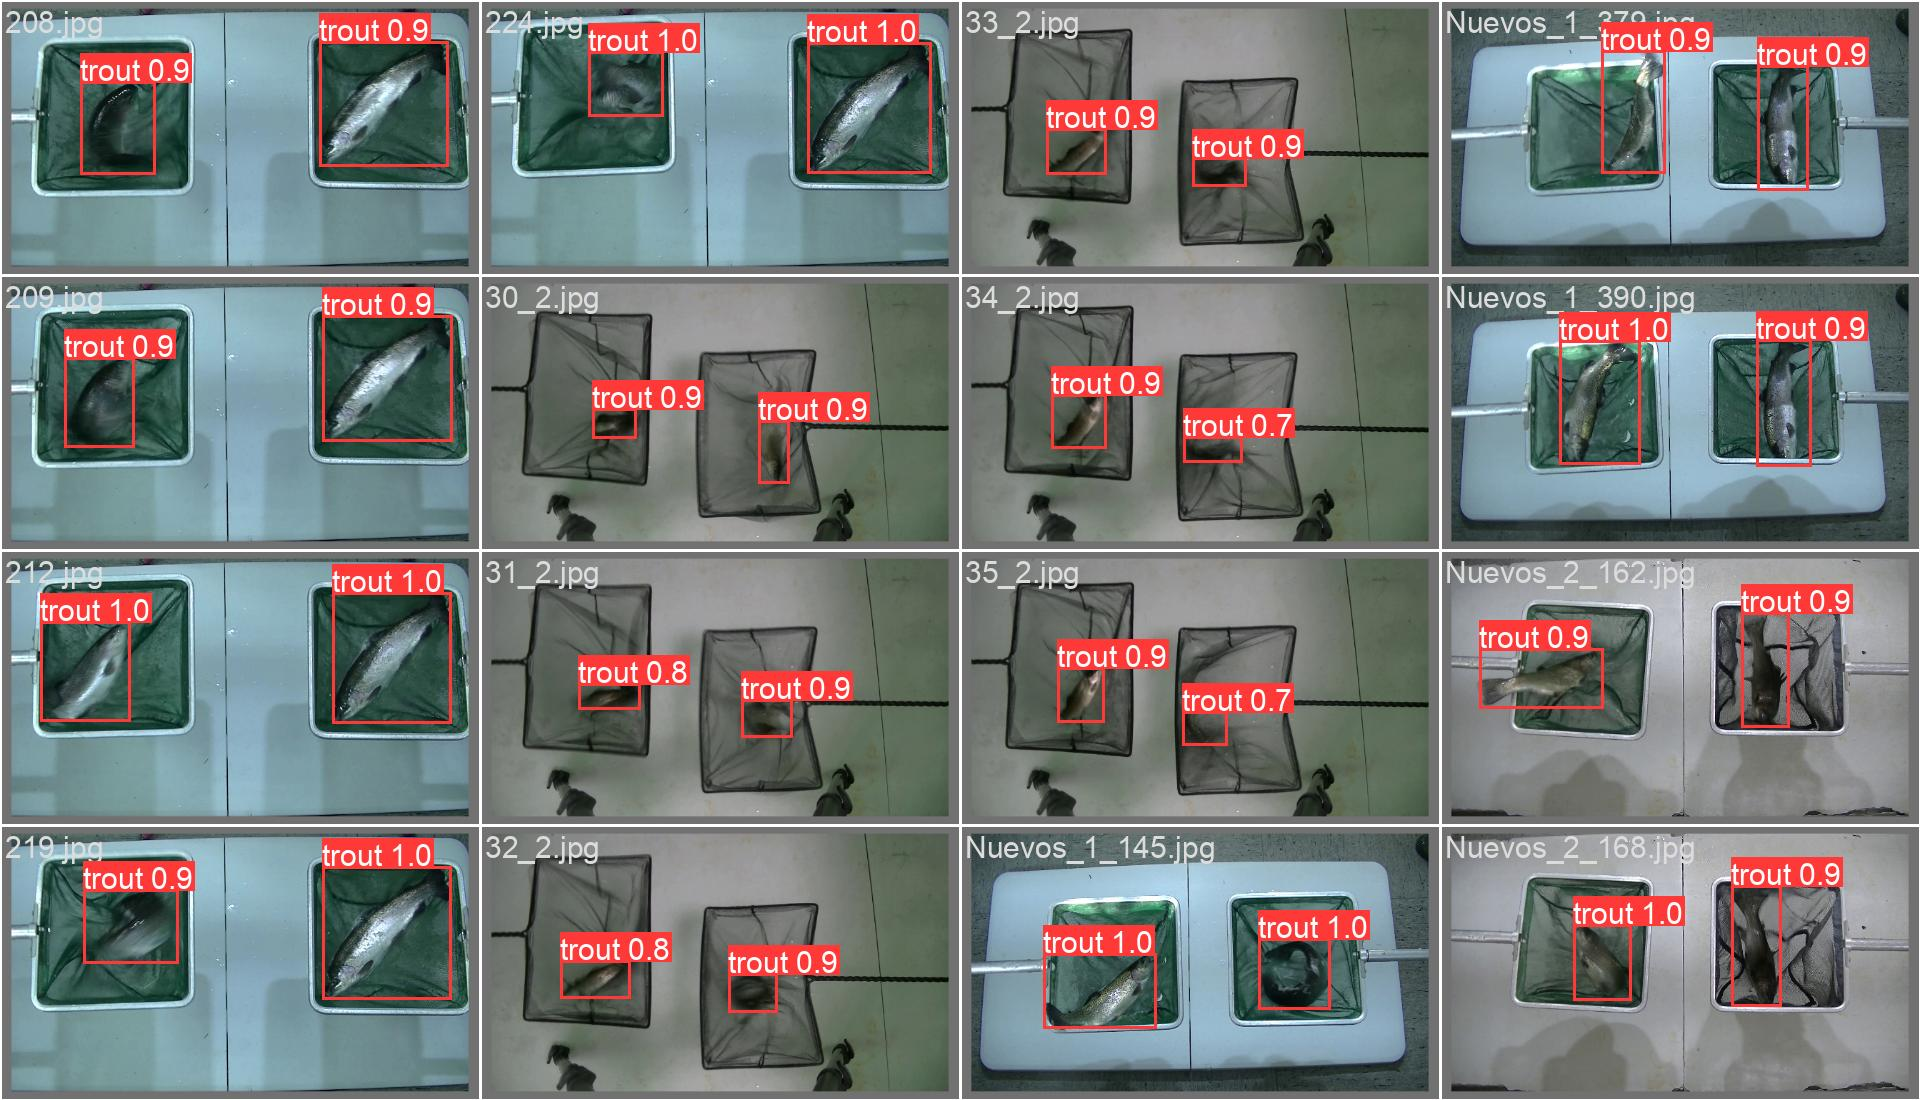
\includegraphics[width=0.95\textwidth]{images/7/pred.jpg}
        \caption{Predicciones sobre el conjunto de validación final}
    \end{subfigure}
    \caption{Resultados finales sobre el conjunto de validación}
    \label{fig:ValidacionRed}
\end{figure}

Aparte de los resultados de validación, como ya se ha dicho en el trabajo y se puede ver en \hyperref[train:final]{las gráficas de resultados del anexo c}, se buscaba maximizar otras métricas como son 
el \texttt{recall} a niveles altos para obtener una cantidad elevada de verdaderos 
positivos. Finalmente, también se ha conseguido alcanzar una precisión \texttt{mAP50-95} muy elevada (0.82) teniendo en cuenta la variabilidad del conjunto de datos, lo cual nos indica una precisión 
general de la red muy buena.

\clearpage

Seguidamente, se realizó la validación del número de movimientos utilizando las etiquetas proporcionadas por los investigadores como ya se comentó en el análisis de los datos. Para esto, se utilizó la aplicación en el conjunto de 
videos del \textit{NetText}1 al \textit{NetText}4, a través de las jaulas 1 a la 4, excluyendo los videos que contenían el primer y el segundo pez (ya que para entrenamiento se han usado los videos \verb|23_NT_R1_J1_P1_2|, \verb|23_NT_R2_J1_P1_P2|, \verb|23_NT_R3_J1_P1_P2| 
y \verb|23_NT_R3_J2_P1_P2|).

Al principio de este trabajo, se pensó que las etiquetas de los investigadores eran incorrectas, ya que al revisar manualmente el movimiento de los videos, el número de movimientos no era ni cercano. Sin embargo, según se realizaba el 
análisis de los videos, se observó que extrañamente, las etiquetas asociadas a la trucha izquierda eran más similares a los movimientos de la derecha y viceversa.

Analizando los coeficientes de correlación y graficando la relación lineal de los datos de la \autoref{fig:EtiquetadosMal}, se observó que efectivamente, los datos etiquetados simplemente no estaban en \acrshort{ltr}, sino al revés. Por lo tanto se arreglaron 
los datos para la .

\begin{figure}[H]
    \centering
    \begin{subfigure}[b]{0.7\textwidth}
        \centering
        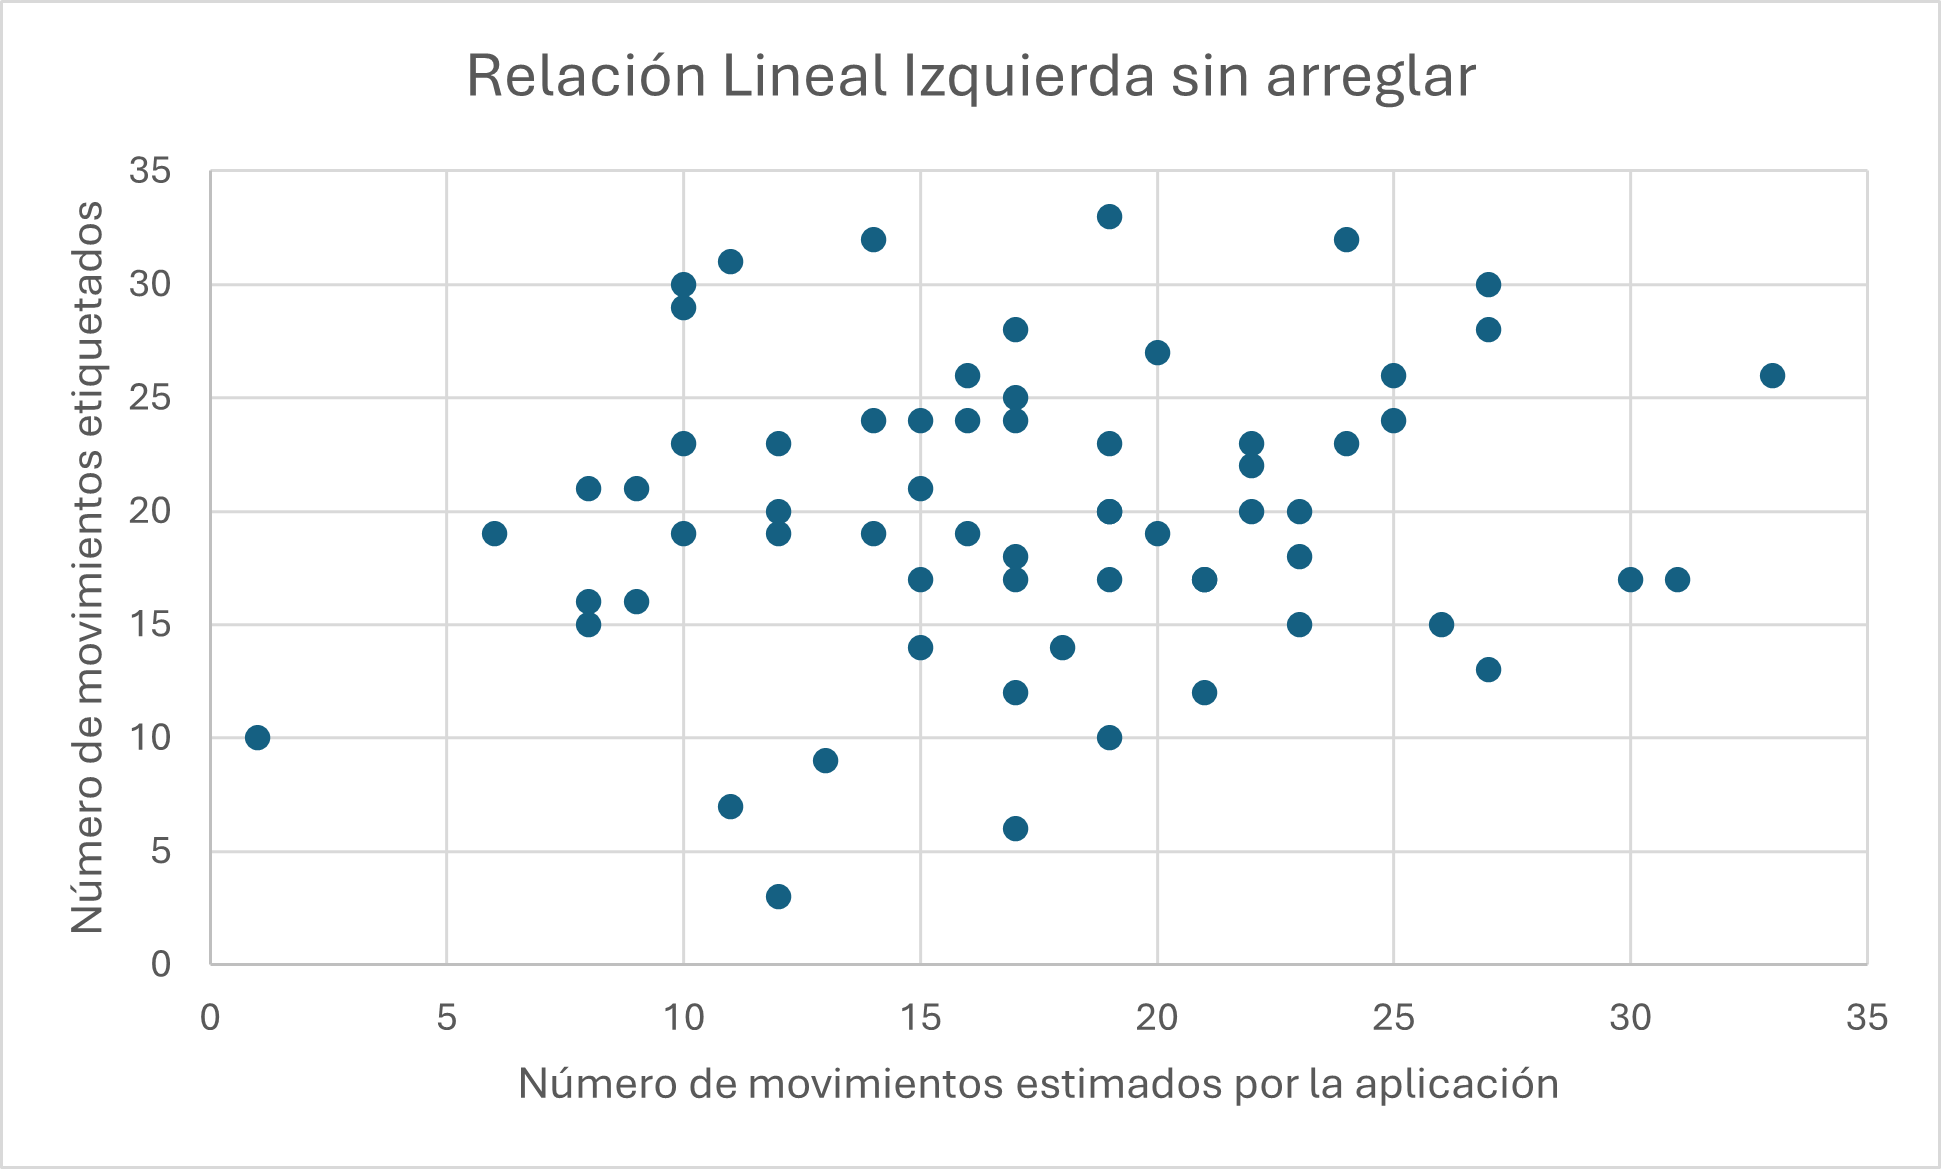
\includegraphics[width=0.9\textwidth]{images/7/IzquierdaMal.png}
        \caption{Relación lineal de los movimientos estimados y etiquetados en la izquierda sin el arreglo(Coeficiente R = 0,154365645)}
    \end{subfigure}
    \begin{subfigure}[b]{0.7\textwidth}
        \centering
        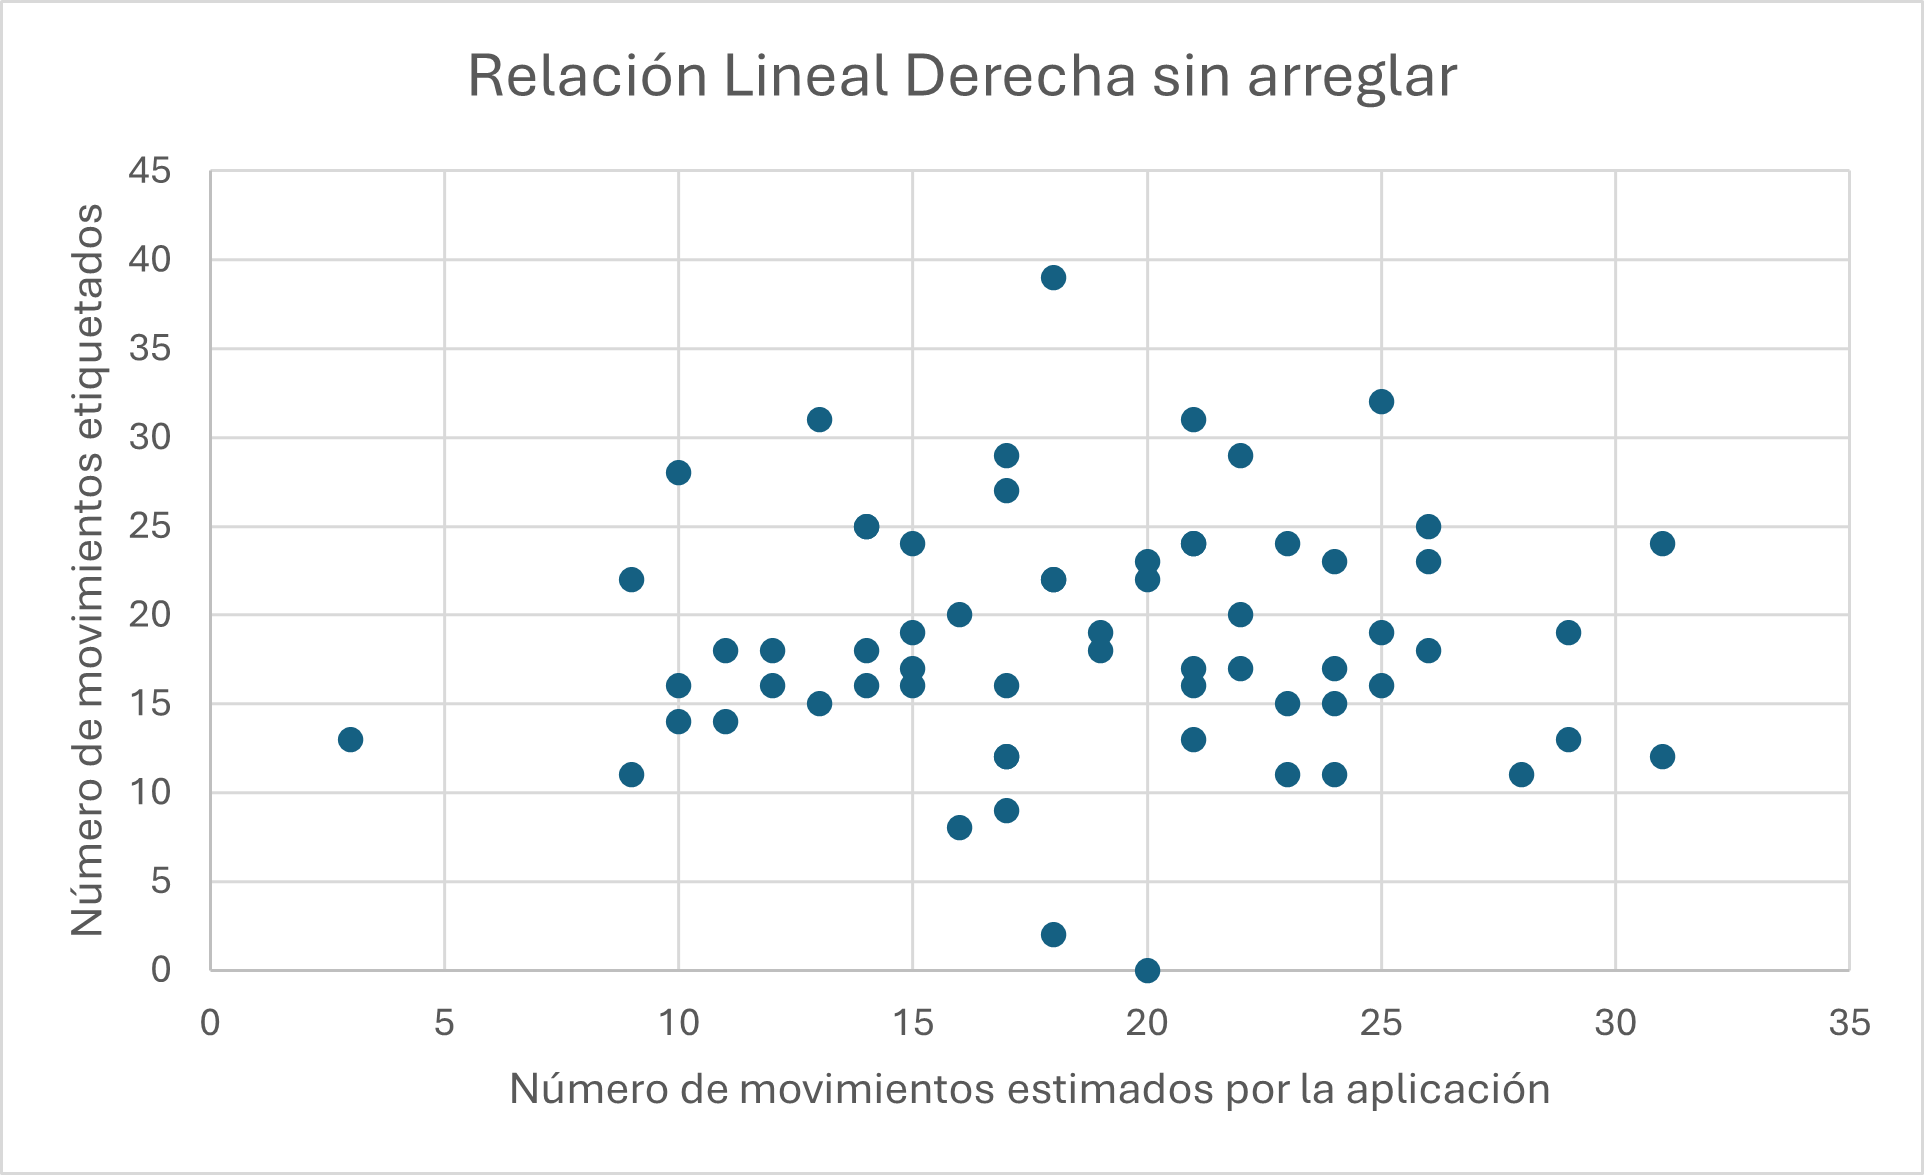
\includegraphics[width=0.9\textwidth]{images/7/DerechaMal.png}
        \caption{Relación lineal de los movimientos estimados y etiquetados en la derecha sin el arreglo(Coeficiente R = 0,032476833)}
    \end{subfigure}
    \caption{Relación de los datos estimados con los etiquetados asumiendo \texttt{LTR}}
    \label{fig:EtiquetadosMal}
\end{figure}

\begin{figure}[H]
    \centering
    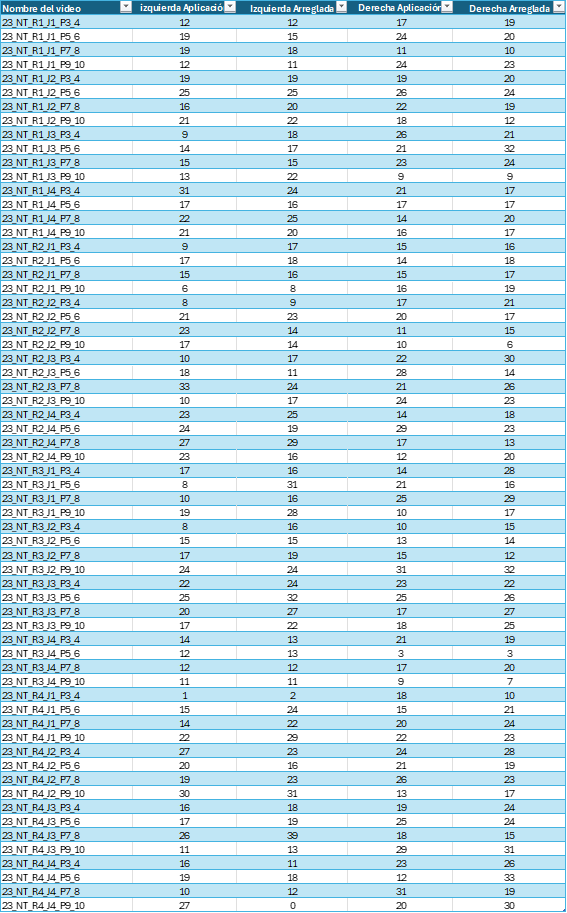
\includegraphics[width=0.85\textwidth]{images/7/ValidacionMovimientos.png}
    \caption{Tabla comparativa entre movimientos estimados y movimientos etiquetados por los investigadores}
    \label{fig:TablaResultados}
\end{figure}
\clearpage
Si se calcula según el arreglo de los datos, se obtienen las gráficas de la \autoref{fig:EtiquetadosBien}, donde se puede observar que la correlación de la aplicación y el algoritmo desarrollado es muy bueno para ser una primera versión.

\begin{figure}[H]
    \centering
    \begin{subfigure}[b]{0.7\textwidth}
        \centering
        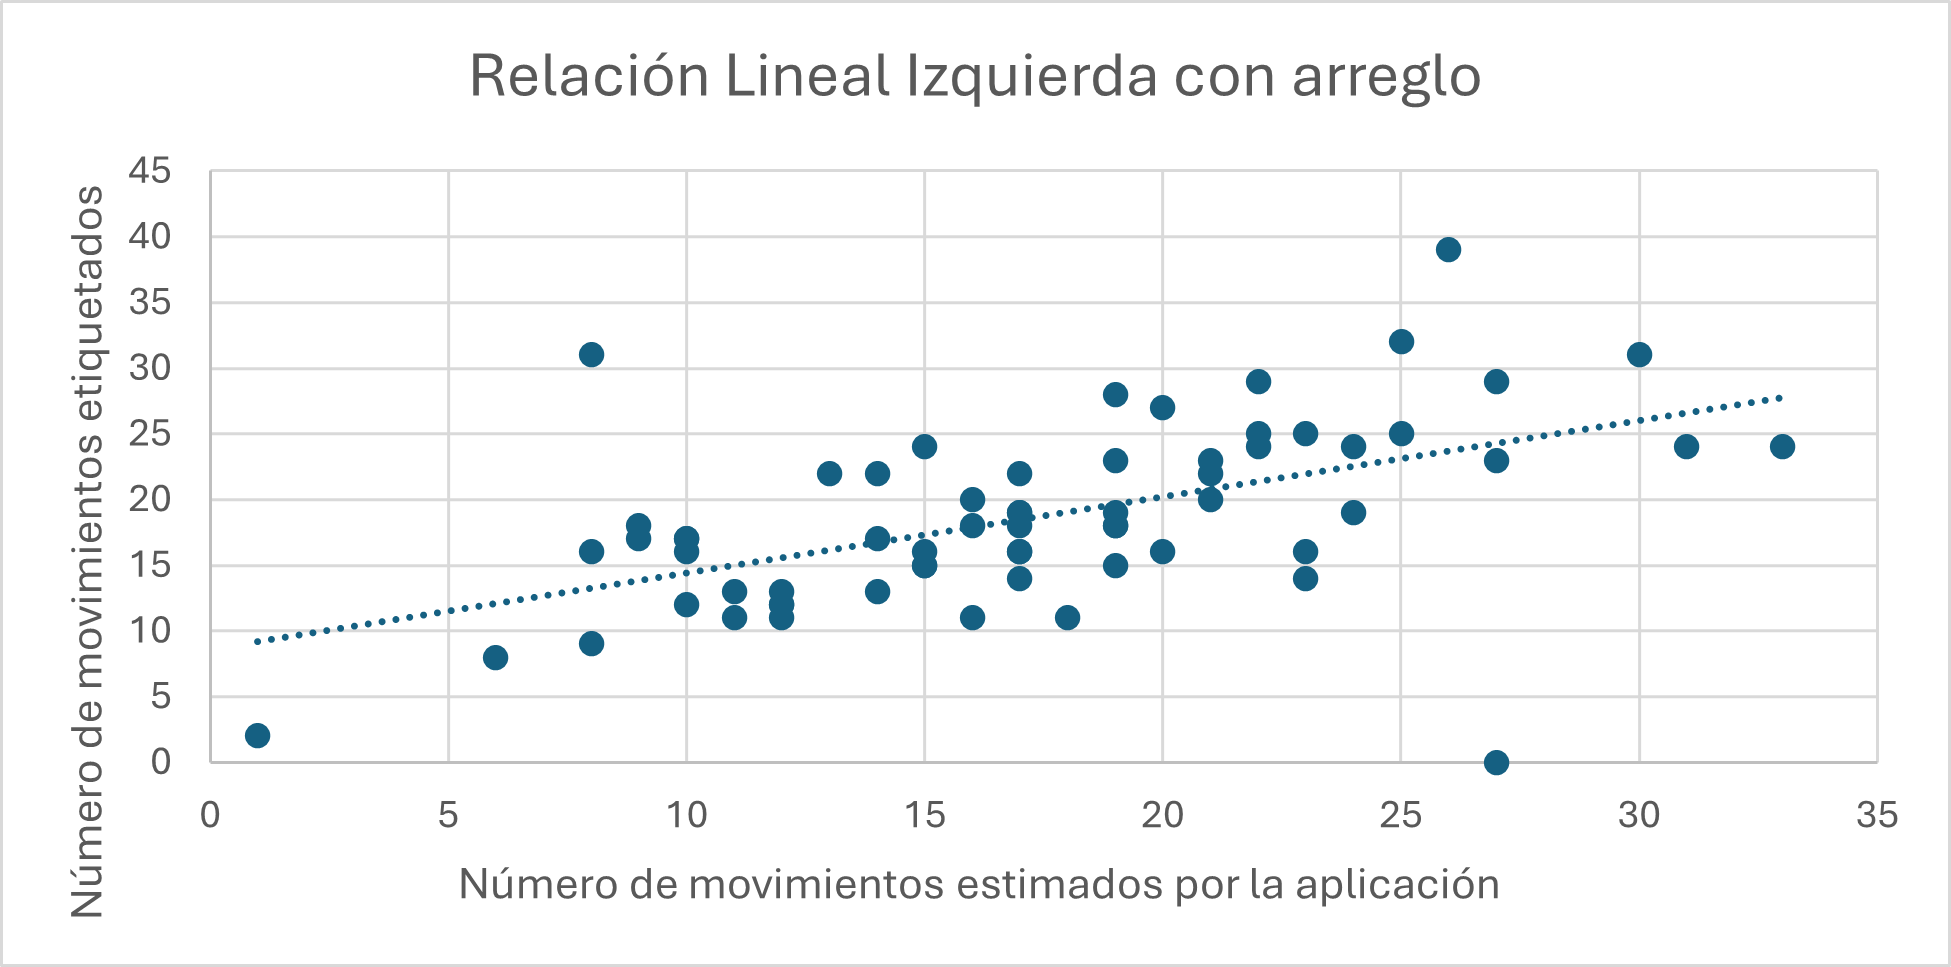
\includegraphics[width=0.9\textwidth]{images/7/IzquierdaBien.png}
        \caption{Relación lineal de los movimientos estimados y etiquetados en la izquierda con el arreglo(Coeficiente R = 0,539455863)}
    \end{subfigure}
    \begin{subfigure}[b]{0.7\textwidth}
        \centering
        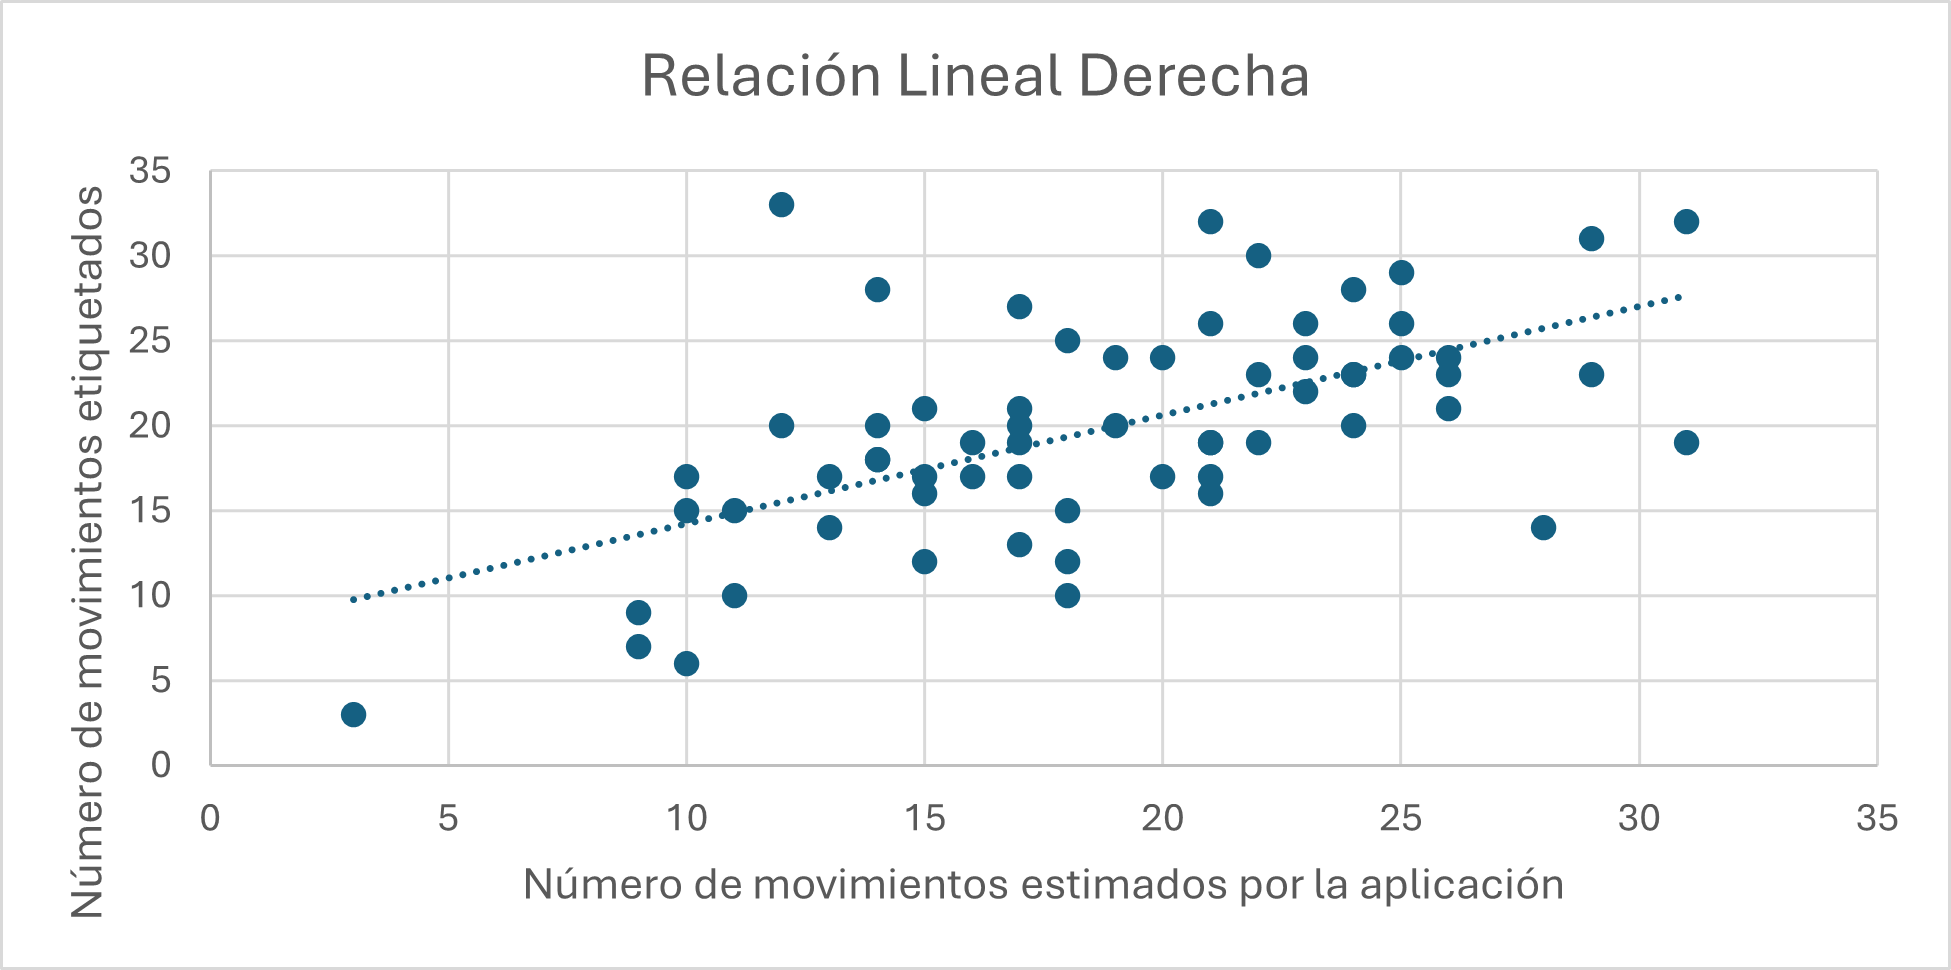
\includegraphics[width=0.9\textwidth]{images/7/DerechaBien.png}
        \caption{Relación lineal de los movimientos estimados y etiquetados en la derecha con el arreglo(Coeficiente R = 0,584222239)}
    \end{subfigure}
    \caption{Relación de los datos estimados con los etiquetados aplicando el arreglo}
    \label{fig:EtiquetadosBien}
\end{figure}
\vspace{3\baselineskip}
Finalmente, se ha calculado los respectivos histogramas de la \autoref{fig:HistogramasError}, en donde se puede observar la distribución del error en la validación. Se puede observar que la mayor parte del error está entre -20\% y el 30\%.

\begin{figure}[H]
    \centering
    \begin{subfigure}[b]{0.7\textwidth}
        \centering
        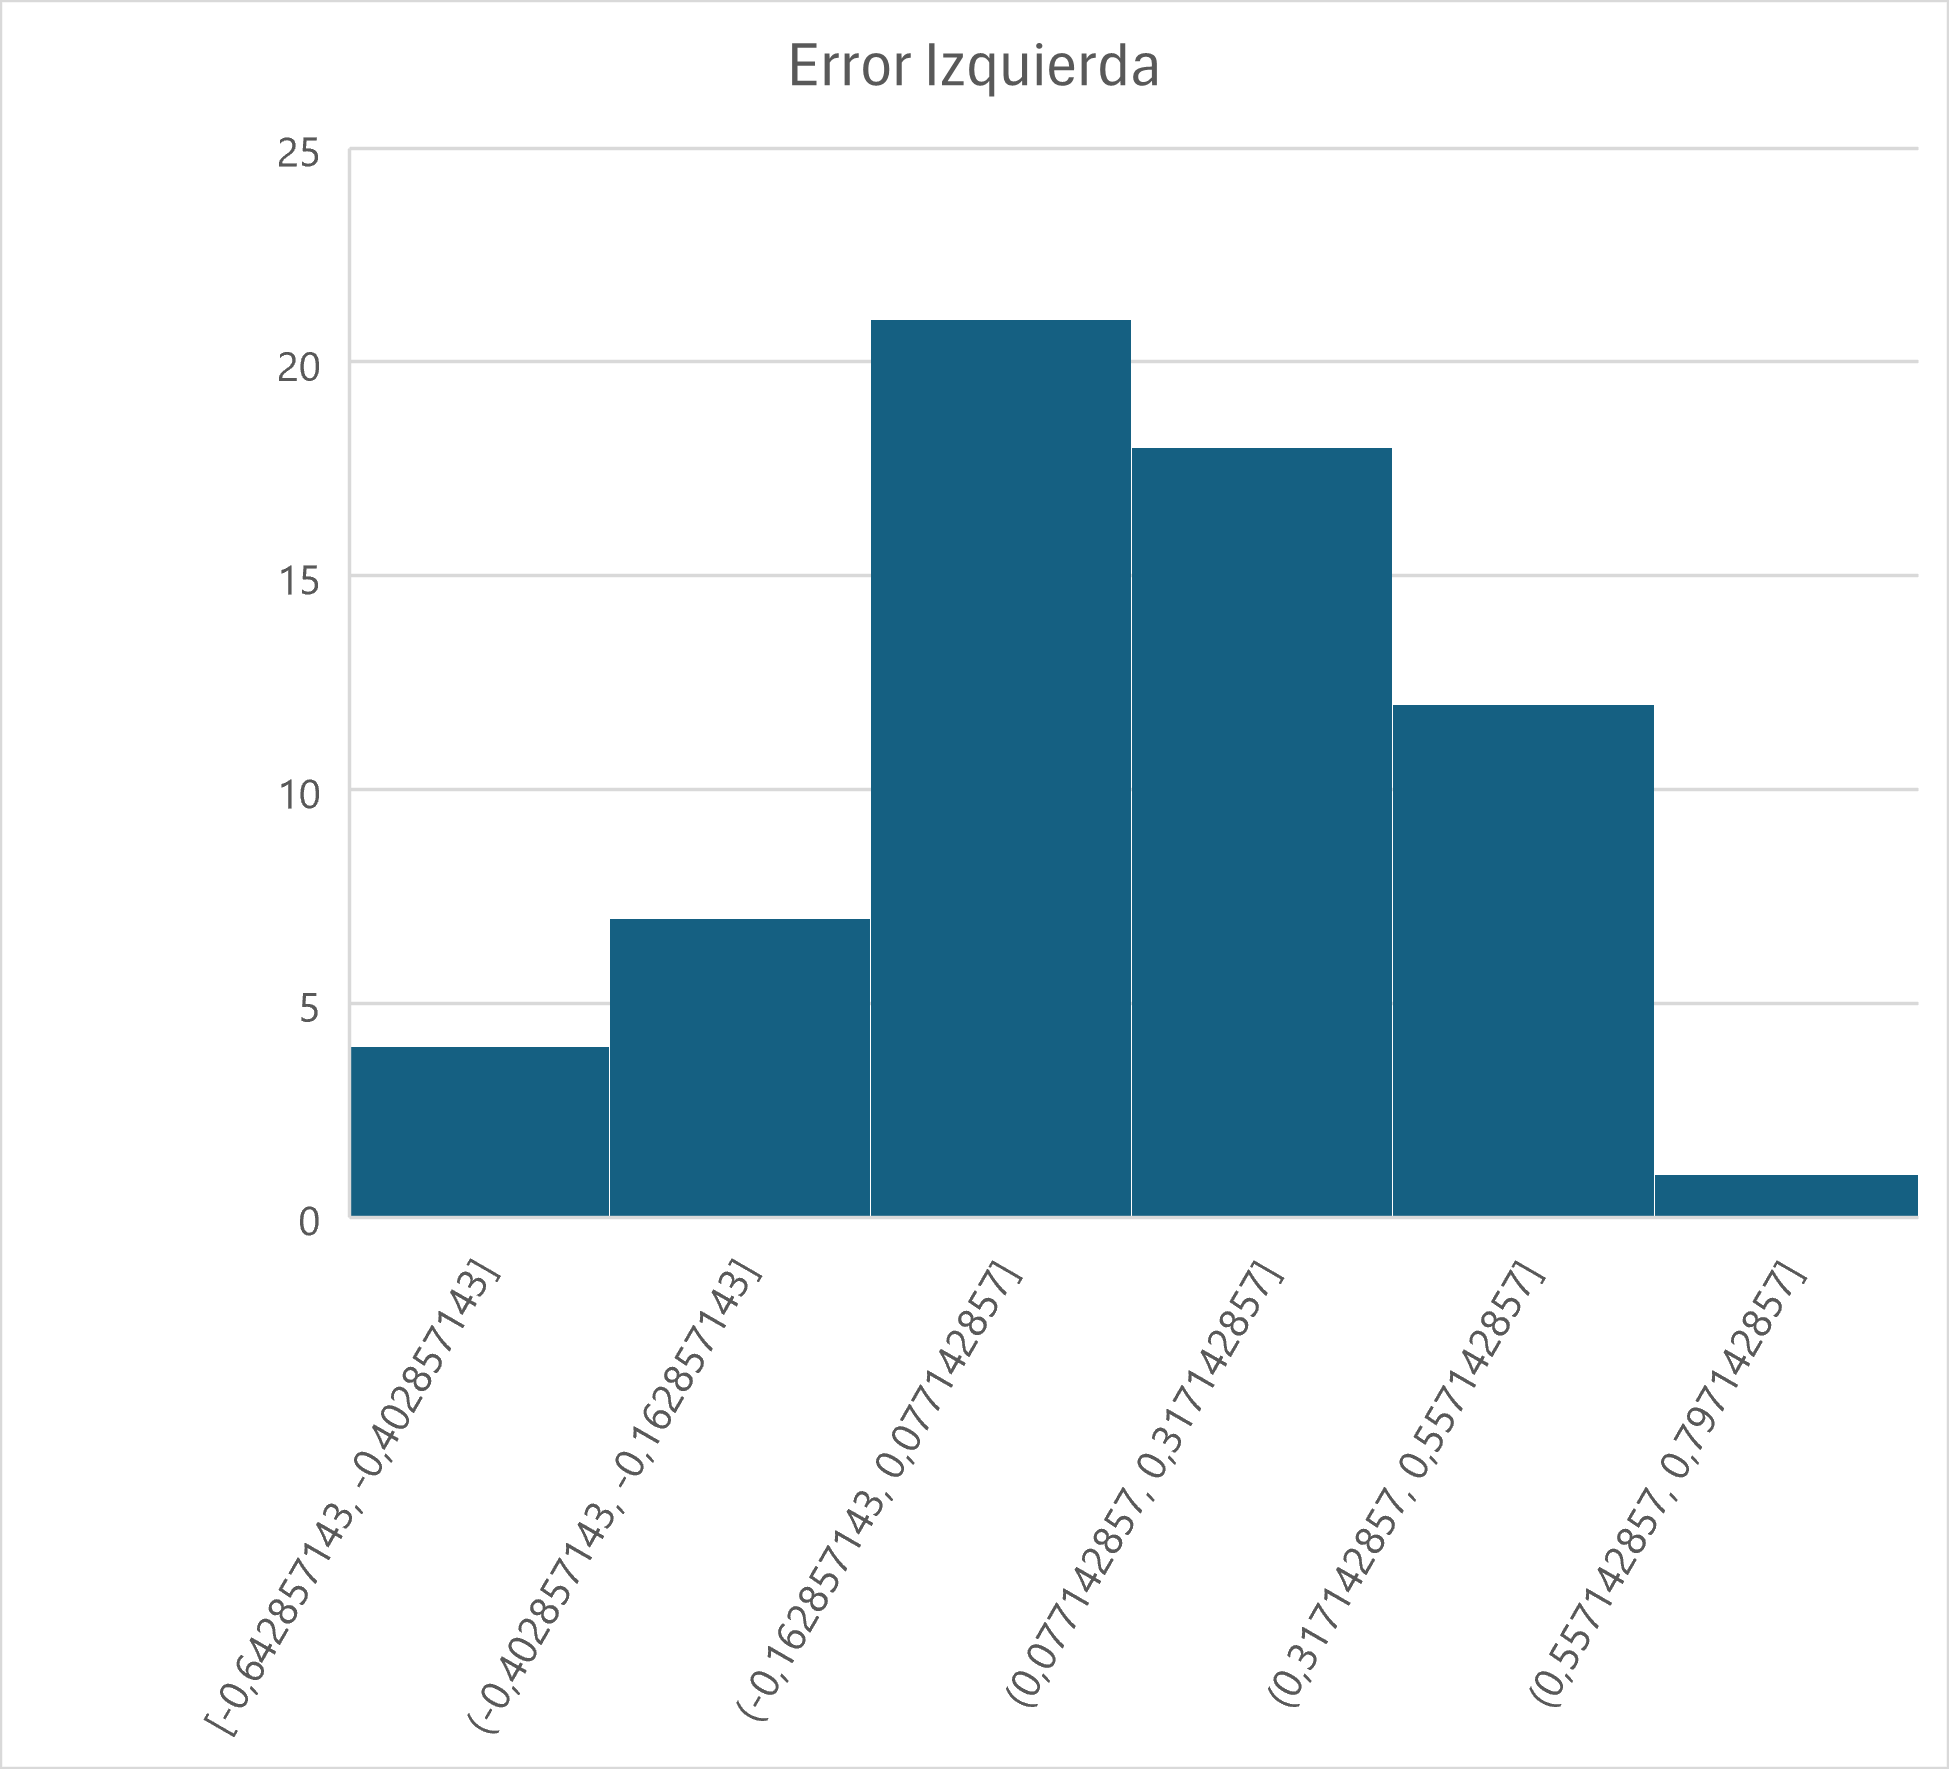
\includegraphics[width=0.9\textwidth]{images/7/ErrorIzquierda.png}
        \caption{Distribución del error en las truchas de la izquierda en validación de resultados}
    \end{subfigure}
    \begin{subfigure}[b]{0.7\textwidth}
        \centering
        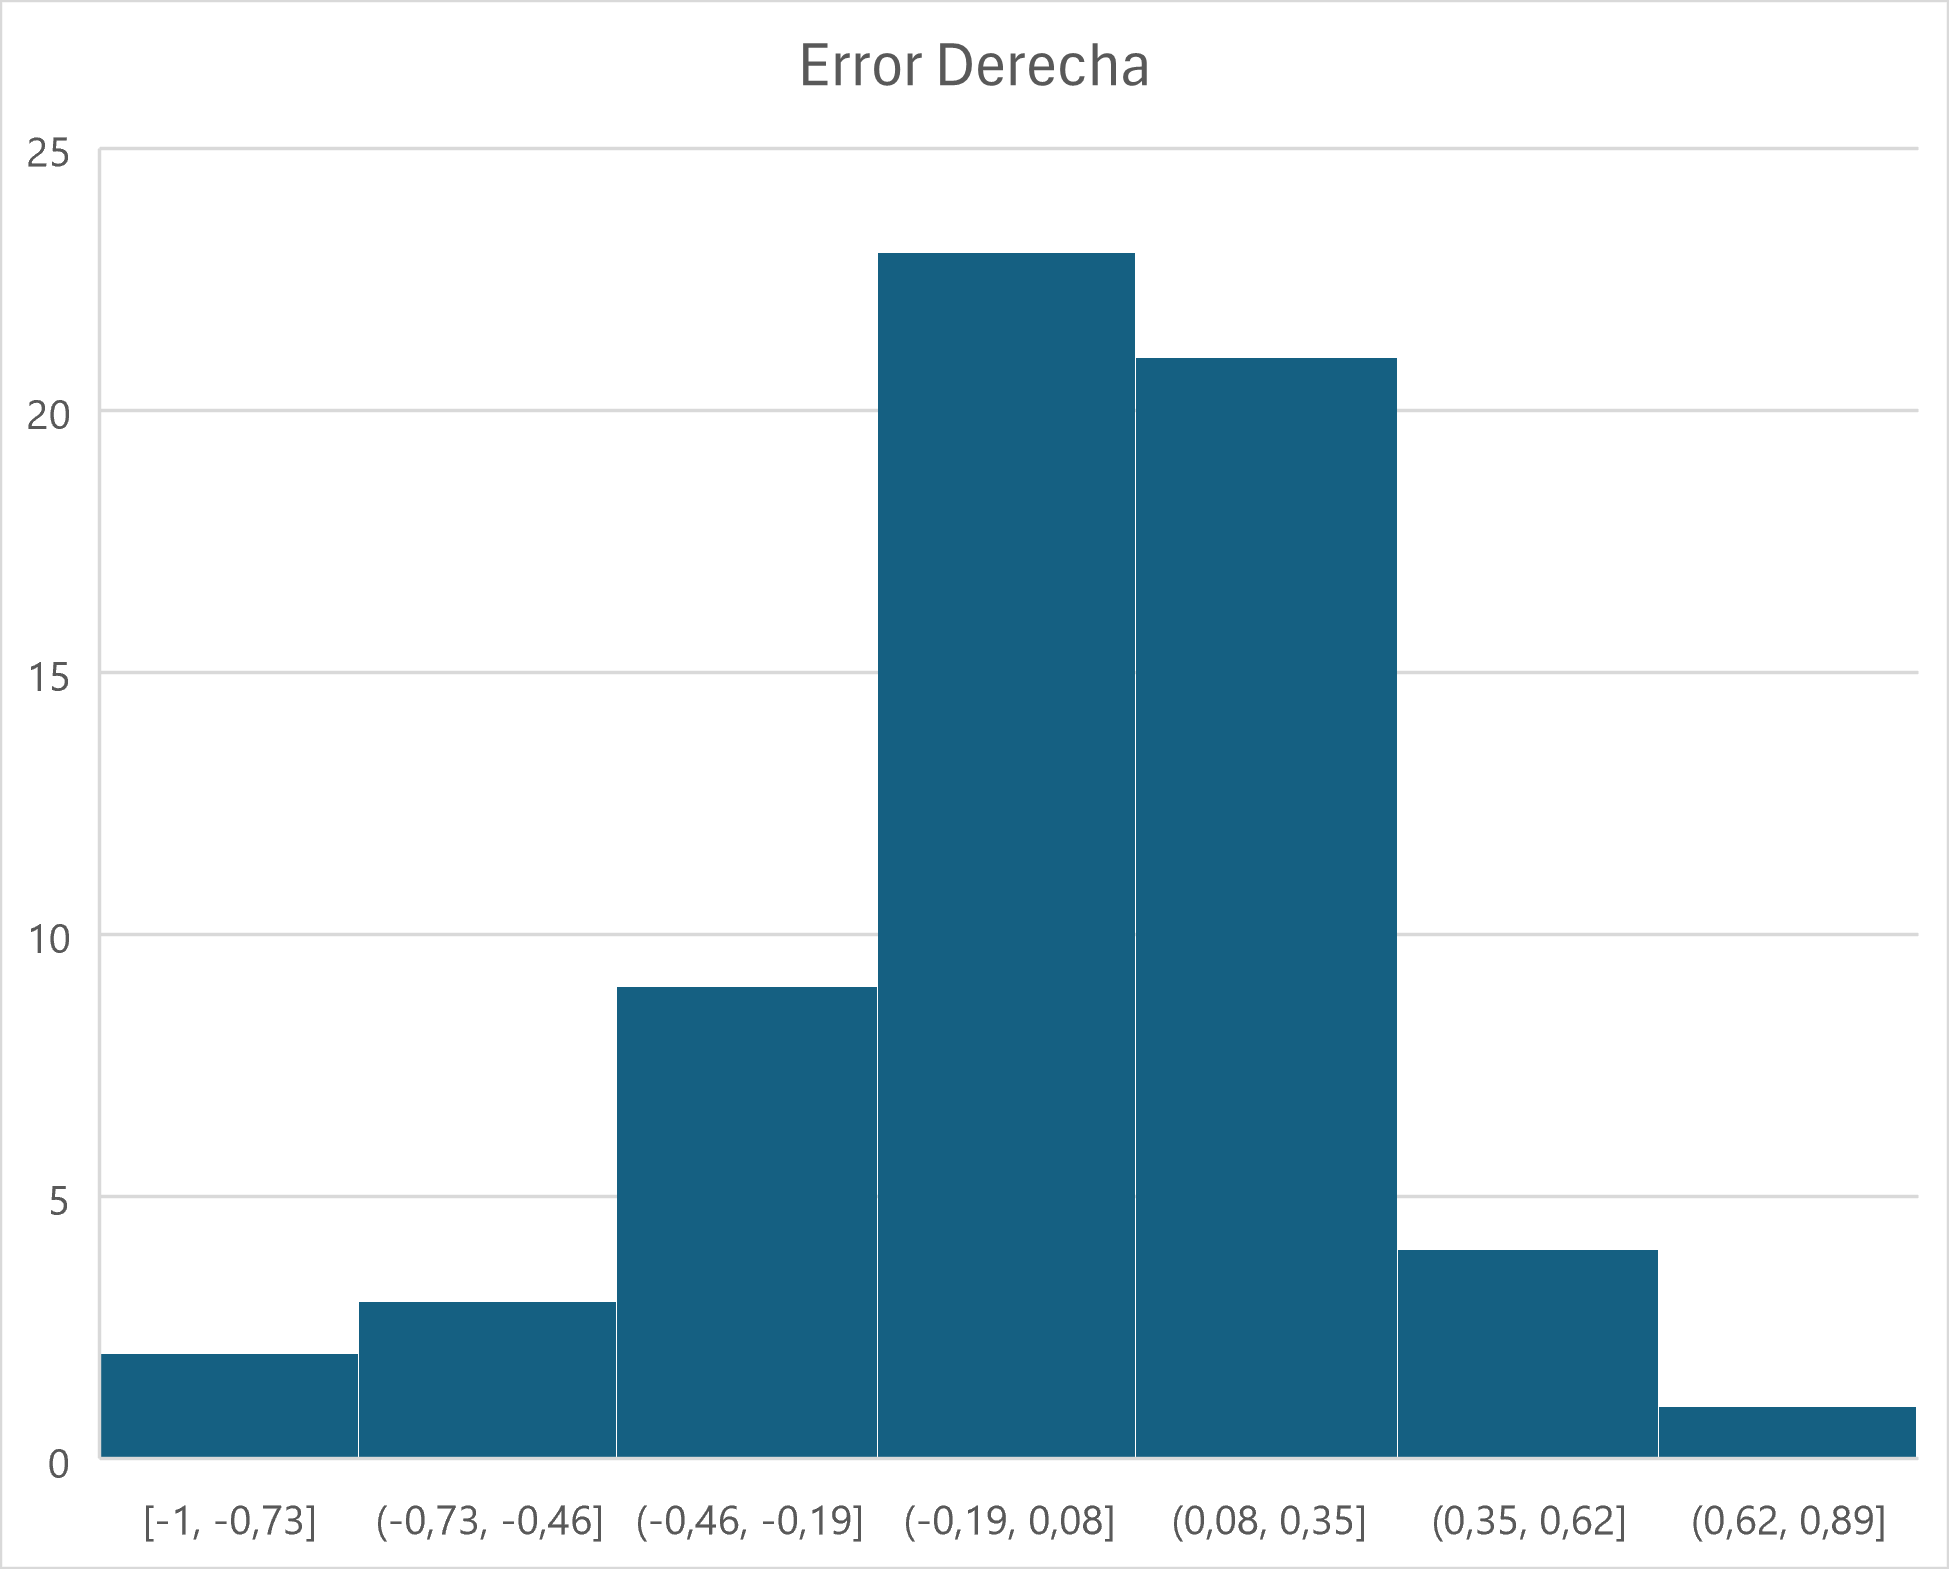
\includegraphics[width=0.9\textwidth]{images/7/ErrorDerecha.png}
        \caption{Distribución del error en las truchas de la derecha en validación de resultados}
    \end{subfigure}
    \caption{Distribución del error respecto a las etiquetas de los investigadores}
    \label{fig:HistogramasError}
\end{figure}

Como resumen, la detección y el conteo de movimiento se ha hecho correctamente, si bien hay errores que pueden provenir de diversos factores como la subjetividad del etiquetado manual y falta de ajuste del algoritmo de conteo 
de movimientos de la aplicación. Sin embargo, como primera aproximación al problema permite ver fácilmente el comportamiento de las truchas de manera comparativa en el \textit{NetTest}.

\clearpage

La última validación de resultados que falta es la relacionada con el rendimiento de la aplicación y el uso del \texttt{HardWare}. En este sentido:

\begin{itemize}
    \item Se ha conseguido una aplicación que consigue seleccionar el mejor formato de red neuronal según el ordenador en el que se ejecute, permitiendo minimizar el tiempo necesario para procesar un video. Esto se ve reflejado en 
    los anteriores resultados, en los que se han procesado 64 videos de 15 segundos cada uno en solo 1 hora en total.
    \item A través de \texttt{DearPyGUI}, se consigue una aplicación fluida que mantiene una tasa de fotogramas sin caídas, lo que provee una experiencia muy buena al usuario.
    \item A través del uso de procesos, se ha conseguido descargar el hilo principal, minimizar tiempos de proceso e implementar funciones multimedia sin que afecte al rendimiento. Esto se ve reflejado en la carga que tiene la 
    aplicación sobre la memoria \texttt{RAM}, que en las pruebas no ha superado el umbral de \texttt{1.5GB} en ningún momento para videos de resolución \texttt{1080P}.
\end{itemize}
